% ============================================================================
%  Defence presentation: "Evaluating Coding Agent Quality: Application to
%  Software Design Principles". Akram Ben Fekih, ISSAT Sousse, 2025/2026.
%
%  Build (MiKTeX, XeLaTeX):   latexmk -xelatex main.tex
%
%  Every number is taken from thesis/latex/chapters/*.tex, which
%  vibebench/07_verify/verify_thesis_numbers.py checks against the data.
%  Figures are the thesis figures, \input from ../latex/figures and typeset in
%  the thesis serif font so their checked spacing is unchanged.
%  Do not load enumitem: it breaks beamer's list labels.
% ============================================================================
\documentclass[11pt,aspectratio=169]{beamer}

\usepackage{fontspec}
\setmainfont{Latin Modern Roman}
\IfFontExistsTF{Segoe UI}{\setsansfont{Segoe UI}[BoldFont={Segoe UI Semibold}]}{%
  \setsansfont{Latin Modern Sans}}
\IfFontExistsTF{Consolas}{\setmonofont{Consolas}[Scale=0.86]}{\setmonofont{Latin Modern Mono}}
\renewcommand{\familydefault}{\sfdefault}

\usepackage{tikz}
\usetikzlibrary{arrows.meta,positioning,shapes.geometric,fit,backgrounds,calc,
                decorations.pathreplacing,shadows}
\usepackage{pgfplots}
\pgfplotsset{compat=1.18}
\usepackage{booktabs}
\usepackage{array}
\usepackage[table]{xcolor}
\usepackage{amsmath,amssymb}

\definecolor{issatblue}{RGB}{7,45,90}
\definecolor{issatgold}{RGB}{176,141,60}
\definecolor{accentgray}{RGB}{90,90,90}
\definecolor{lightblue}{RGB}{223,232,242}
\definecolor{darktext}{RGB}{38,38,40}
\definecolor{srpcolor}{RGB}{31,119,180}
\definecolor{ocpcolor}{RGB}{255,127,14}
\definecolor{lspcolor}{RGB}{44,160,44}
\definecolor{ispcolor}{RGB}{214,39,40}
\definecolor{dipcolor}{RGB}{148,103,189}

\newcolumntype{L}[1]{>{\raggedright\arraybackslash}p{#1}}

\usetheme{default}
\setbeamertemplate{navigation symbols}{}
\setbeamercolor{normal text}{fg=darktext}
\setbeamercolor{structure}{fg=issatblue}
\setbeamerfont{frametitle}{size=\large,series=\bfseries}
\setbeamercolor{frametitle}{fg=issatblue,bg=white}
\setbeamertemplate{frametitle}{%
  \vspace{7pt}%
  {\usebeamerfont{frametitle}\usebeamercolor[fg]{frametitle}\insertframetitle}\par
  \vspace{-3pt}{\color{issatgold}\rule{\textwidth}{1.1pt}}\par\vspace{3pt}}
\setbeamertemplate{itemize item}{\color{issatgold}\small\textbullet}
\setbeamertemplate{itemize subitem}{\color{accentgray}\small\textendash}
\setbeamercolor{block title}{bg=lightblue,fg=issatblue}
\setbeamercolor{block body}{bg=lightblue!35,fg=darktext}
\setbeamertemplate{blocks}[rounded]
\setbeamertemplate{footline}{%
  \hspace{12pt}{\color{accentgray}\tiny Evaluating Coding Agent Quality}\hfill
  {\color{accentgray}\scriptsize\insertframenumber\,/\,\inserttotalframenumber}\hspace{12pt}\vspace{5pt}}

% figure from the thesis, in the thesis font, scaled to a height or width
\newcommand{\thesisfigH}[2]{{\rmfamily\resizebox{!}{#1}{\input{../latex/figures/#2.tex}}}}
\newcommand{\thesisfigW}[2]{{\rmfamily\resizebox{#1}{!}{\input{../latex/figures/#2.tex}}}}
% a number with a caption
\newcommand{\keynum}[3][2.6cm]{%
  \begin{tikzpicture}[baseline]
    \node[draw=issatblue,line width=0.9pt,rounded corners=4pt,fill=lightblue!55,
          inner sep=5pt,align=center,text width=#1]
      {{\large\bfseries\color{issatblue}#2}\\[1pt]{\scriptsize\color{accentgray}#3}};
  \end{tikzpicture}}
\newcommand{\takeaway}[1]{%
  \begin{tikzpicture}
    \node[fill=issatgold!18,draw=issatgold!80!black,rounded corners=4pt,inner sep=6pt,
          text width=0.95\textwidth,align=left,font=\small] {#1};
  \end{tikzpicture}}

\title{Evaluating Coding Agent Quality}
\subtitle{Application to Software Design Principles}
\author{Akram Ben Fekih}
\date{2025/2026}

\begin{document}

% ============================================================== 1 title
\begin{frame}[plain]
\begin{tikzpicture}[remember picture,overlay]
  \node[anchor=north west] at ([xshift=0.6cm,yshift=-0.45cm]current page.north west)
    {
\includegraphics[height=1.1cm]{../latex/front/logos/issat.jpg}};
  \node[anchor=north] at ([yshift=-0.45cm]current page.north)
    {
\includegraphics[height=1.0cm]{../latex/front/logos/ministry.jpg}};
  \node[anchor=north east] at ([xshift=-0.6cm,yshift=-0.45cm]current page.north east)
    {
\includegraphics[height=1.0cm]{../latex/front/logos/sousse.png}};
\end{tikzpicture}
\vspace{1.35cm}
\begin{center}
{\small\color{accentgray} Research Master's in Computer Science, Intelligent Pervasive Systems}\\[10pt]
{\LARGE\bfseries\color{issatblue} Evaluating Coding Agent Quality}\\[4pt]
{\large\color{accentgray} Application to Software Design Principles}\\[10pt]
{\color{issatgold}\rule{0.5\textwidth}{1.2pt}}\\[10pt]
{\large Akram Ben Fekih}\\[2pt]
{\small Supervised by Mrs.\ Maha Khemaja}\\[2pt]
{\footnotesize\color{accentgray} ISSAT Sousse, University of Sousse \ $\cdot$ \ 2025/2026}
\end{center}
\end{frame}

% ============================================================== 2 context
\begin{frame}{Coding agents now submit real changes}
\begin{columns}[T,onlytextwidth]
\begin{column}{0.56\textwidth}
\begin{itemize}\setlength{\itemsep}{5pt}
  \item Agents such as \textbf{Claude Code}, \textbf{GitHub Copilot} and \textbf{OpenAI Codex}
        take a task and open a pull request.
  \item The AIDev dataset records \textbf{7.69 million} agent pull requests in 957k repositories.
  \item They are evaluated mainly on whether tests pass (HumanEval, SWE-bench).
  \item Passing tests says little about \textbf{design}: whether the next developer can change
        the code.
\end{itemize}
\end{column}
\begin{column}{0.4\textwidth}
\keynum[4.6cm]{about half}{of SWE-bench Verified patches that pass the tests would not be merged
by maintainers (METR, 2026)}\\[6pt]
\keynum[4.6cm]{77\%}{of long-horizon agent trajectories show growing structural erosion
(SlopCodeBench, 2026)}
\end{column}
\end{columns}
\end{frame}

% ============================================================== 3 gap
\begin{frame}{What is missing}
\begin{columns}[T,onlytextwidth]
\begin{column}{0.5\textwidth}
\textbf{Existing studies}
\begin{itemize}\setlength{\itemsep}{3pt}
  \item Benchmarks on functions or small sets of tasks
  \item LLMs as SOLID detectors on examples, not on agent output
  \item Smell counts on merged code only
  \item Metrics assumed to capture a principle, rarely validated
\end{itemize}
\end{column}
\begin{column}{0.47\textwidth}
\textbf{This thesis}
\begin{itemize}\setlength{\itemsep}{3pt}
  \item Real pull requests from three agents
  \item All five SOLID principles
  \item Merged, rejected \emph{and} open requests
  \item Each detector's precision and recall \textbf{measured}
  \item Full replication in a second language
\end{itemize}
\end{column}
\end{columns}
\end{frame}

% ============================================================== 4 RQs
\begin{frame}{Research questions}
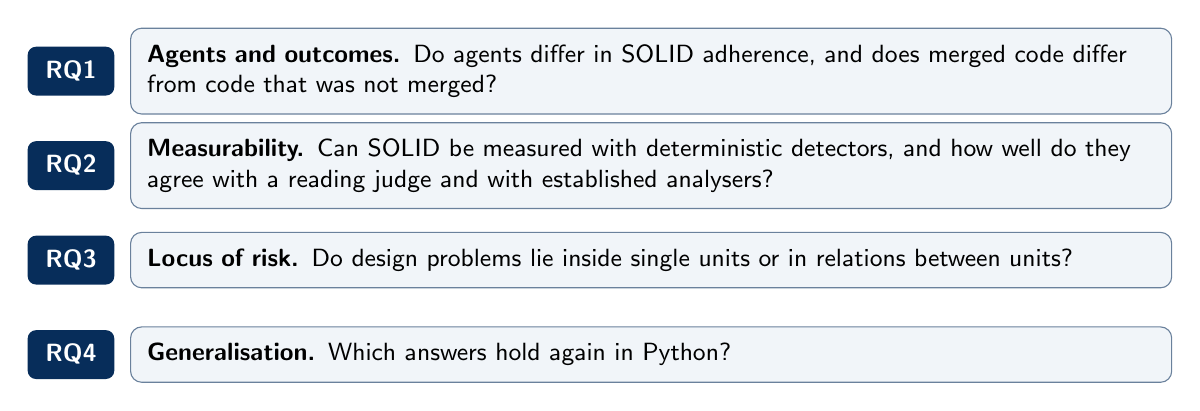
\begin{tikzpicture}[
  q/.style={draw=issatblue!60,fill=lightblue!45,rounded corners=4pt,text width=12.8cm,
            inner sep=6pt,align=left,font=\small},
  tag/.style={fill=issatblue,text=white,rounded corners=3pt,font=\small\bfseries,
              minimum width=1.1cm,minimum height=0.62cm},
]
\foreach \y/\t/\q in {0/RQ1/{\textbf{Agents and outcomes.} Do agents differ in SOLID adherence, and does
merged code differ from code that was not merged?},
-1.2/RQ2/{\textbf{Measurability.} Can SOLID be measured with deterministic detectors, and how well
do they agree with a reading judge and with established analysers?},
-2.4/RQ3/{\textbf{Locus of risk.} Do design problems lie inside single units or in relations
between units?},
-3.6/RQ4/{\textbf{Generalisation.} Which answers hold again in Python?}}{
  \node[tag] (t) at (0,\y) {\t};
  \node[q,anchor=west] at (0.75,\y) {\q};
}
\end{tikzpicture}
\end{frame}

% ============================================================== 5 SOLID
\begin{frame}{Five principles, five detectors}
\begin{center}
\thesisfigW{0.92\textwidth}{fig_solid_wheel}
\end{center}
\vspace{-2pt}
{\small Each detector looks for the structure a violation usually leaves in the code.}
\end{frame}

% ============================================================== 6 pipeline
\begin{frame}{Method}
\begin{center}
\thesisfigH{0.8\textheight}{fig_pipeline}
\end{center}
\end{frame}

% ============================================================== 7 corpus
\begin{frame}{Corpus}
\begin{columns}[T,onlytextwidth]
\begin{column}{0.48\textwidth}
\centering
\keynum[2.55cm]{4,245}{Java PRs\\1,010 repositories}\hspace{4pt}%
\keynum[2.55cm]{4,946}{Python PRs\\2,921 repositories}\\[10pt]
\begin{itemize}\setlength{\itemsep}{3pt}
  \item Same three agents in both languages
  \item Balanced on agent $\times$ outcome
  \item $\geq$25 stars, permissive licence
  \item Python sample stratified by repository
\end{itemize}
\end{column}
\begin{column}{0.48\textwidth}
\begin{block}{Rejected is not refused}
Only requests with a review record a judgement about the code.\\[3pt]
Java: 171 of 1,177 unmerged requests were reviewed.\\
Python: 196 of 1,496.\\[3pt]
Outcomes are therefore compared by stratum, and only where both sides were reconstructed the same
way.
\end{block}
\end{column}
\end{columns}
\end{frame}

% ============================================================== 8 delta
\begin{frame}{Charging only what the pull request changed}
\begin{center}
\thesisfigW{0.93\textwidth}{fig_delta_harness}
\end{center}
{\small For a relation-level principle, a violation is charged when either side of the relation is
in a touched file.}
\end{frame}

% ============================================================== 9 validation design
\begin{frame}{How the detectors were validated}
\begin{columns}[T,onlytextwidth]
\begin{column}{0.52\textwidth}
\begin{itemize}\setlength{\itemsep}{4pt}
  \item 100 flagged + 100 unflagged entities per principle
  \item A reading judge (LLM) labels each one, \textbf{with a reason}, without seeing the verdict
  \item An audit gate: every label traces to the source shown
  \item Recall weighted by stratum size
  \item Holdout samples for the two refinements
  \item DIP (Java) and ISP (Python): every flag judged
\end{itemize}
\end{column}
\begin{column}{0.44\textwidth}
\centering
\keynum[4.2cm]{2,475}{entities judged\\1,495 Java, 980 Python}\\[8pt]
\keynum[4.2cm]{89.7\%}{agreement when 174 Java entities were judged twice}\\[8pt]
\keynum[4.2cm]{0.966 $\rightarrow$ 0.352}{Liskov recall, unweighted vs weighted}
\end{column}
\end{columns}
\end{frame}

% ============================================================== 10 RQ2 validity
\begin{frame}{RQ2: how faithful are the detectors?}
\begin{center}
\thesisfigH{0.72\textheight}{fig_validation_pr}
\end{center}
\vspace{-4pt}
{\small Dependency Inversion is precise in both languages (0.892 Java, 1.000 Python). SRP, OCP and
ISP are screens: most flags do not survive reading.}
\end{frame}

% ============================================================== 11 refinements
\begin{frame}{RQ2: a shape rule transfers, a tuned number does not}
\begin{center}
\small
\begin{tabular}{@{}lccc@{}}
\toprule
\textbf{Refinement} & \textbf{Derivation sample} & \textbf{Java holdout} & \textbf{Python (unchanged)} \\
\midrule
LSP, refused bequest only & 1.000 (31/31) & \textbf{1.000} (33/33) & \textbf{0.857} (6/7) \\
ISP, $\geq$30 members & 0.862 (25/29) & 0.704 (19/27) & 0.200 (1/5) \\
\bottomrule
\end{tabular}
\end{center}
\vspace{6pt}
\begin{columns}[T,onlytextwidth]
\begin{column}{0.48\textwidth}
\begin{itemize}\setlength{\itemsep}{3pt}
  \item Refused bequest is \textbf{categorical}: a method body is only a throw, or it is not.
  \item The width of 30 was chosen where false positives stopped, and absorbed sample noise.
\end{itemize}
\end{column}
\begin{column}{0.48\textwidth}
\begin{itemize}\setlength{\itemsep}{3pt}
  \item In Python, 46 of the 51 confirmed Liskov violations rest on faults \texttt{javac} would
        reject: the compiler decides which faults can exist.
\end{itemize}
\end{column}
\end{columns}
\end{frame}

% ============================================================== 12 external tools
\begin{frame}{RQ2: agreement with published analysers (Java)}
\begin{columns}[T,onlytextwidth]
\begin{column}{0.55\textwidth}
\small
\begin{tabular}{@{}lc@{}}
\toprule
\textbf{God Class detectors, 82,553 types} & \textbf{Cohen's $\kappa$} \\
\midrule
ours vs PMD \texttt{GodClass} & 0.574 \\
ours vs DesigniteJava & 0.531 \\
PMD vs DesigniteJava & 0.384 \\
\bottomrule
\end{tabular}\\[8pt]
\begin{tabular}{@{}lc@{}}
\toprule
\textbf{Rank correlation with CK} & \textbf{$\rho$} \\
\midrule
weighted methods & 0.977 \\
lines of code & 0.944 \\
cohesion (LCOM1) & 0.288 \\
\bottomrule
\end{tabular}
\end{column}
\begin{column}{0.41\textwidth}
\begin{itemize}\setlength{\itemsep}{4pt}
  \item 150 random repositories, default thresholds
  \item The rubric agrees with each tool more than the tools agree with each other
  \item 68.0\% of our flags confirmed by at least one tool
  \item Cohesion metrics disagree everywhere, including within CK
\end{itemize}
\end{column}
\end{columns}
\end{frame}

% ============================================================== 13 size
\begin{frame}{RQ1: raw rates mostly measure change size}
\begin{columns}[T,onlytextwidth]
\begin{column}{0.5\textwidth}
\small
Mean Java files per pull request:\\[3pt]
Claude Code \textbf{46.4} \quad Copilot \textbf{18.5} \quad Codex \textbf{10.9}\\[8pt]
\begin{tabular}{@{}llccc@{}}
\toprule
& \textbf{Files} & \textbf{Claude} & \textbf{Copilot} & \textbf{Codex} \\
\midrule
OCP & 1--3 & 1.3\% & \textbf{1.9\%} & 0.4\% \\
    & 11+  & \textbf{31.3\%} & 19.3\% & 8.9\% \\
DIP & 1--3 & 0.4\% & 0.5\% & \textbf{0.8\%} \\
    & 11+  & \textbf{22.3\%} & 13.7\% & 12.1\% \\
\bottomrule
\end{tabular}
\end{column}
\begin{column}{0.46\textwidth}
\begin{itemize}\setlength{\itemsep}{4pt}
  \item Claude Code has the highest pooled rate on all five principles.
  \item The ordering holds on large changes and breaks on small ones.
  \item So the agents must be compared \textbf{at the same change size}.
\end{itemize}
\end{column}
\end{columns}
\end{frame}

% ============================================================== 14 model
\begin{frame}{RQ1: the joint model}
\begin{columns}[T,onlytextwidth]
\begin{column}{0.54\textwidth}
\small
Per principle: agent + $\log$(files) + month,\\GEE clustered by repository.\\[6pt]
\footnotesize
\begin{tabular}{@{}lcc@{}}
\toprule
& \textbf{Java} & \textbf{Python} \\
\midrule
odds per doubling of files & 1.88--1.95 & 2.01--2.18 \\
Claude Code, OCP & 2.22 & 2.09 \\
\quad 95\% interval & 1.21--4.07 & 1.44--3.04 \\
\quad $p$ & 0.010 & 0.0001 \\
time, per month & $\approx$1 & $\approx$1 \\
\bottomrule
\end{tabular}\\[3pt]
{\scriptsize\color{accentgray} odds ratios against Copilot; time for the delta principles}
\end{column}
\begin{column}{0.42\textwidth}
\begin{itemize}\setlength{\itemsep}{4pt}
  \item \textbf{Change size dominates} in both languages.
  \item \textbf{One agent difference replicates}: Claude Code on Open/Closed.
  \item It passes Bonferroni in Python; Java alone does not, so the claim rests on replication.
  \item Python's import-cycle effect (1.88, $p$ = 0.0096) is not confirmed.
\end{itemize}
\end{column}
\end{columns}
\end{frame}

% ============================================================== 15 outcomes
\begin{frame}{RQ1: merged against unmerged code}
\begin{columns}[T,onlytextwidth]
\begin{column}{0.47\textwidth}
\small
\textbf{Java}, tier-matched\\[3pt]
\footnotesize
\begin{tabular}{@{}lrcc@{}}
\toprule
\textbf{Stratum} & \textbf{n} & \textbf{OCP} & \textbf{DIP} \\
\midrule
merged & 1,521 & 8.3\% & 4.6\% \\
unreviewed & 1,006 & 7.5\% & 5.6\% \\
reviewed, closed & 135 & 12.6\% & 12.6\% \\
\bottomrule
\end{tabular}\\[6pt]
\small Merged $\approx$ unreviewed.
\end{column}
\begin{column}{0.47\textwidth}
\small
\textbf{Python}, tier-matched\\[3pt]
\footnotesize
\begin{tabular}{@{}lrcc@{}}
\toprule
\textbf{Stratum} & \textbf{n} & \textbf{OCP} & \textbf{DIP} \\
\midrule
merged & 1,734 & 4.9\% & 3.1\% \\
unreviewed & 1,300 & 9.1\% & 4.5\% \\
reviewed, closed & 163 & 7.4\% & 8.6\% \\
\bottomrule
\end{tabular}\\[6pt]
\small Merged is cleaner: unmerged odds 1.57 (OCP) and 2.43 (LSP) after size and agent.
\end{column}
\end{columns}
\vspace{8pt}
\takeaway{The languages disagree. Most unmerged requests were never reviewed, so neither result shows
what reviewers select on.}
\end{frame}

% ============================================================== 16 locus
\begin{frame}{RQ3: where the problems live}
\begin{center}
\thesisfigW{0.9\textwidth}{fig_intra_inter}
\end{center}
\end{frame}

\begin{frame}{RQ3: most violations were already there}
\begin{center}
\thesisfigH{0.66\textheight}{fig_present_introduced}
\end{center}
\vspace{-4pt}
{\small Refused bequest: 183 present vs 16 introducing PRs in Java, 176 vs 5 in Python. Between 0.4\%
and 4.1\% of Java pull requests introduce a violation.}
\end{frame}

% ============================================================== 18 authored
\begin{frame}{RQ3: agent-written classes are flagged less}
\begin{center}
\thesisfigW{0.92\textwidth}{fig_srp_agents}
\end{center}
\vspace{-2pt}
{\small Pooled: 7.7\% vs 13.5\% in Java, 8.9\% vs 12.1\% in Python. The groups differ in age and size,
so this describes the corpus; it does not rank agents against people.}
\end{frame}

% ============================================================== 19 RQ4
\begin{frame}{RQ4: what generalises}
\small
\begin{tabular}{@{}L{5.0cm}L{3.9cm}L{4.4cm}@{}}
\toprule
\textbf{Result} & \textbf{Java} & \textbf{Python} \\
\midrule
Change size dominates & OR 1.88--1.95 & \textcolor{lspcolor!70!black}{\textbf{holds}} 2.01--2.18 \\
Claude Code on Open/Closed & 2.22 (1.21--4.07) & \textcolor{lspcolor!70!black}{\textbf{holds}} 2.09 (1.44--3.04) \\
Present far exceeds introduced & 183 vs 16 & \textcolor{lspcolor!70!black}{\textbf{holds}} 176 vs 5 \\
Authored flagged less than edited & 7.7\% vs 13.5\% & \textcolor{lspcolor!70!black}{\textbf{holds}} 8.9\% vs 12.1\% \\
Shape rule transfers, number does not & 1.000 vs 0.704 & \textcolor{lspcolor!70!black}{\textbf{holds}} 0.857 vs 0.200 \\
Merged equals unreviewed & yes & \textcolor{ispcolor!80!black}{\textbf{does not hold}} \\
SRP screen precision & 0.350 & \textcolor{ispcolor!80!black}{\textbf{drops}} to 0.110 \\
\bottomrule
\end{tabular}
\end{frame}

% ============================================================== 20 contributions
\begin{frame}{Contributions and practical use}
\begin{columns}[T,onlytextwidth]
\begin{column}{0.5\textwidth}
\textbf{Contributions}
\begin{itemize}\setlength{\itemsep}{3pt}\small
  \item A validated SOLID instrument over real agent pull requests
  \item A corpus with merged, rejected and open requests
  \item A map of which principles a rule measures and which it only screens
  \item Evidence in two languages that most problems predate the agent's change
  \item A replication with the same agents
\end{itemize}
\end{column}
\begin{column}{0.46\textwidth}
\textbf{For a review check}
\begin{itemize}\setlength{\itemsep}{3pt}\small
  \item Add \textbf{refused bequest}: 64/64 in Java, 6/7 in Python
  \item In dynamic languages, also check that overrides accept the base's calls
  \item Do not rely on interface-width thresholds
  \item Treat SRP and OCP flags as prompts for discussion
\end{itemize}
\end{column}
\end{columns}
\end{frame}

% ============================================================== 21 limitations
\begin{frame}{Limitations}
\begin{columns}[T,onlytextwidth]
\begin{column}{0.49\textwidth}
\begin{itemize}\setlength{\itemsep}{3pt}\small
  \item SOLID adherence is not measured design quality or cost
  \item Labels come from an LLM judge of the same family as one agent
  \item No independent-tool check for OCP, ISP or Python
  \item Agents chose their tasks: associations, not causes
\end{itemize}
\end{column}
\begin{column}{0.49\textwidth}
\begin{itemize}\setlength{\itemsep}{3pt}\small
  \item Few reviewed rejections (171 Java, 196 Python)
  \item One snapshot per pull request, no long-term erosion
  \item Both corpora from one dataset; 7.0\% of Python source lost
  \item Small counts for relation-level principles
\end{itemize}
\end{column}
\end{columns}
\end{frame}

% ============================================================== 22 conclusion
\begin{frame}{Conclusion and future work}
\takeaway{Most design problems in the code these agents touch were there before them; how much an
agent changes matters more than which agent it is. Both results hold in Java and in Python.}
\vspace{8pt}
\begin{columns}[T,onlytextwidth]
\begin{column}{0.49\textwidth}
\textbf{Next steps}
\begin{itemize}\setlength{\itemsep}{2pt}\small
  \item Recognise closed sets from external specifications (OCP)
  \item Compare OCP with DesigniteJava's type-conditional smells
  \item Re-judge Python samples; a second judge
\end{itemize}
\end{column}
\begin{column}{0.49\textwidth}
\vspace{16pt}
\begin{itemize}\setlength{\itemsep}{2pt}\small
  \item A corpus with many reviewed rejections
  \item Repository history as the unit of analysis
  \item A third language with structural typing
\end{itemize}
\end{column}
\end{columns}
\end{frame}

% ============================================================== 23 thanks
\begin{frame}[plain]
\vfill
\begin{center}
{\LARGE\bfseries\color{issatblue} Thank you}\\[8pt]
{\color{issatgold}\rule{0.35\textwidth}{1.2pt}}\\[8pt]
{\large Questions}
\end{center}
\vfill
\end{frame}

\end{document}
